\bookchapter{第四十九章：搭建開發環境——Android Studio與第一個項目}

\chapterintro{工欲善其事，必先利其器。此章吾儕將「廚房」搭好：裝好Android Studio、跑通模擬器、創建人生第一個安卓項目，再將工程結構拆開看個明白。裝好環境之後，汝會第一次看到自己寫之代碼變成一個能點之按鈕——此一瞬間，甚多人會記一輩子。}

\booksection{一、安裝Android Studio}

Android Studio乃谷歌官方之集成開發環境（IDE），免費，功能全家桶：寫代碼、看界面預覽、調試、打包全於其中。安裝四步：

\begin{enumerate}
  \item 打開官網developer.android.com/studio，下載最新穩定版（2026年8月乃Narwhal之後之版本，Windows/Mac/Linux皆有）；
  \item 運行安裝包，一路「下一步」——安裝嚮導會自動帶上Android SDK與模擬器組件；
  \item 首次啟動時按提示下載SDK組件（默認勾選就好，可能須幾分鐘與幾個GB之空間）；
  \item 完成後汝會看到歡迎頁——恭喜，「廚房」搭好了。
\end{enumerate}

\begin{tcbwarn}{注意：硬件要求心裡有數}
Android Studio乃一個「喫記憶體」之傢夥：建議16GB記憶體起步（8GB也能跑，但模擬器一開則比較卡）、磁盤預留20GB以上、CPU支持虛擬化（BIOS裡開啟VT-x/AMD-V）。若電腦確實老舊，可用「真機調試」代替模擬器（本章第四節會講），體驗反而更流暢。

\end{tcbwarn}

\booksection{二、創建汝之第一個項目}

於歡迎頁點New Project，選Empty Activity模板（最乾淨之新手模板），然後填三樣東西：

\begin{center}
\begin{tabularx}{\linewidth}{|X|X|X|}
\hline
\textbf{配置項} & \textbf{填何} & \textbf{說明} \tabularnewline
\hline
Name & My First App & 應用名字，顯示於手機桌面上 \tabularnewline
Package name & com.example.myfirstapp & 全球唯一標識，習慣乃「域名反寫」，先按默認 \tabularnewline
Minimum SDK & API 26（Android 8.0） & 最低支持版本，覆蓋95\%以上設備 \tabularnewline
\hline
\end{tabularx}
\end{center}

\begin{center}\small\color{gray}創建項目要填之三件事\end{center}

點Finish後，Android Studio會用Gradle自動下載依賴、構建項目（第一次要等幾分鐘，之後每次會快甚多）。構建完成後，汝就有了一個能跑之App——雖然它還只會顯示一行「Hello Android!」。

\begin{tcbinfo}{小訣：包名之門道}
包名（package name）就像App之「身份證號」，全球不能重複，上架後就不能改了。個人練習用com.example.xxx就行；正式產品要換成汝自己之域名反寫（譬如com.汝之名.應用名）。勿用com.example上架——商店會拒收。

\end{tcbinfo}

\booksection{三、跑起來：模擬器與真機}

代碼寫好了，得尋個「手機」來跑。汝有兩個選擇：

\booksubsection{模擬器（Emulator）}

模擬器者，於電腦中虛擬安卓手機一部也。啟 Android Studio，開 Device Manager Create Device，擇一機（宜 Pixel 系列） 選系統影像（取帶 Google APIs 者） 下載 啟動。繼點工具欄綠色三角 Run，俄而數秒，「手機」之屏遂現汝之 App。

\booksubsection{真機調試（尤所薦）}

真機者，至真之試煉之境也——滑動之手感、真網、真感應之器，模擬器皆莫能及。安卓真機調試甚簡：

\begin{enumerate}
  \item 於手機啟［設定］［關於手機］，連點「版本號」七次，則「開發者選項」啟矣；
  \item 於［開發者選項］中啟 USB 調試；
  \item 以數據線連電腦，手機彈窗，擇「允許 USB 調試」；
  \item 返 Android Studio，工具欄設備下拉之列遂現汝機，點 Run。
\end{enumerate}

\textbf{避坑之警：USB 調試勿恆開}\par

USB 調試者，猶為電腦開「後門」也。凡公共之所充電、接不可信之電腦，務閉 USB 調試，以防他人由之竊讀汝之數據。平居開發，用畢即閉，習以為常。

\booksection{四、工程結構拆解：諸文件何所司}

初啟項目，左側文件之樹或令汝目眩。勿慌，日常開發，汝百分之九十惟與下列數者相交接：

\begin{center}
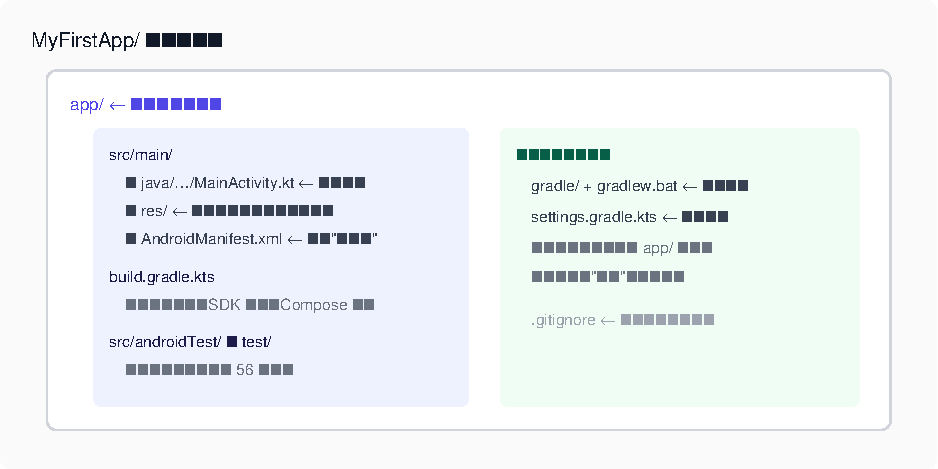
\includegraphics[width=0.92\linewidth]{figures/fig-di-si-shi-jiu-zhang-1}
\\[2pt]\small 圖 2：新手必曉之工程結構（口訣：惟觸 app/ 目錄）
\end{center}

\begin{itemize}
  \item MainActivity.kt：App 之「大門」也。用戶點圖標而啟，首被喚醒者即之。今模板中，其司顯「Hello Android!」之職。
  \item AndroidManifest.xml：App 之「戶口簿」也——聲明此 App 何名、何圖標、有何頁面、需何權限（相機、定位之屬）。
  \item res/ 目錄：資源之倉也，藏圖片、圖標、字符串、顏色。文字置於資源之文件而不硬寫於代碼，乃安卓開發之善習（易語言、易主題皆便）。
  \item build.gradle.kts：構建之方也——聲明最低支持之版本、所倚之庫（如 Compose）。
\end{itemize}

\booksection{五、小試牛刀：易「Hello」為汝名}

啟 MainActivity.kt，則見 Compose 模板所生之代碼。得 Text(“Hello Android!”) 一行，易引號中之字為汝名，如 Text(“汝好，張三！此吾之首個App”)，繼按 Ctrl+R（Mac 則 Cmd+R）復行。數秒之後，模擬器遂顯汝名矣。

\begin{lstlisting}[language=Kotlin]
setContent {
    MyFirstAppTheme {
        Surface(modifier = Modifier.fillMaxSize()) {
            // v 改此為汝之文字
            Text("汝好，張三！此乃吾之首App")
        }
    }
}
\end{lstlisting}

賀矣，汝已竟一全環：「改代碼 編譯 安裝 運行」。此環者，異日日日開發之常也。乘熱打鐵，試更易他者：增字之號、易其色——次章將明此諸「魔法」所自來。

\booksection{六、常見報錯急救：新手前兩週之「急診室」}

環境初建、首次構建之際，汝十有八九將遇下列三種報錯。勿慌，皆有解藥：

\begin{center}
\begin{tabularx}{\linewidth}{|X|X|X|}
\hline
\textbf{報錯之象} & \textbf{常見之因} & \textbf{解藥} \tabularnewline
\hline
Gradle sync failed / 依賴下載遲緩 & 網絡通倉庫不暢 & 為 Gradle 配國內鏡像倉庫（阿里雲/騰訊雲 maven 鏡像），網上搜「gradle 國內鏡像」依而改之 \tabularnewline
SDK 組件缺失 & 安裝時跳過 SDK 之下載 & Settings SDK Manager 補裝所缺之平臺與工具 \tabularnewline
模擬器啟動敗 / 黑屏 & 虛擬化未啟、影像損壞 & BIOS 啟 VT-x/AMD-V；刪模擬器而重建；或逕用真機調試 \tabularnewline
\hline
\end{tabularx}
\end{center}

\begin{center}\small\color{gray}新手環境報錯急救之表\end{center}

\begin{tcbinfo}{小識：搜報錯之法}
報錯之首行最有值——原樣抄入搜索引擎，加以「android studio」之關鍵詞。勿搜「吾環境裝不上奈何」之泛問，當搜「Gradle sync failed: Could not resolve com.android.tools.build」之具體錯。問也精，答方精。

\end{tcbinfo}

\begin{tcbpractice}{來動手：竟汝「開發儀式感」之單}
(1) 裝 Android Studio 且通模擬器；(2) 以真機行己之 App 一遭，截圖以存；(3) 易 Hello 之文為汝名；(4) 壓縮項目而存檔。四步既畢，即可於朋友圈宣曰：吾亦安卓開發者矣（截圖為證）。

\end{tcbpractice}

\begin{tcbsummary}{本章小結}
\begin{itemize}
  \item Android Studio = 官家免費之 IDE；宜 16GB 記憶體 + 20GB 磁盤 + 啟虛擬化
  \item 新建項目三要素：名、包名（舉世唯一，com.example 勿上架）、最低 SDK（自 API 26 始）
  \item 運行之道二：模擬器（電腦中虛擬之機）與真機（啟 USB 調試，用畢記閉）
  \item 工程口訣：惟觸 app/ 目錄——MainActivity.kt 為大門，Manifest 為戶口簿，res/ 為資源之倉
  \item 開發日常 = 改代碼 Run 觀其效，循環往復
\end{itemize}

\end{tcbsummary}
